\documentclass[aspectratio=169]{beamer}
\usetheme{Boadilla}
%\usetheme{Warsaw}
%\setbeamercovered{transparent}
\beamertemplatetransparentcoveredhigh
\usepackage[portuges]{babel}
\usepackage[utf8]{inputenc}
\usepackage{lmodern}
\usepackage[T1]{fontenc}
\usepackage{hyperref} 
\usepackage{listings}

\lstset{frame=tb,
  language=C,
  aboveskip=3mm,
  belowskip=3mm,
  showstringspaces=false,
  columns=flexible,
  basicstyle={\small\ttfamily},
  numbers=none,
  breaklines=true,
  breakatwhitespace=true,
  tabsize=3
}

\newcommand{\eng}[1]{\textsl{#1}}
\newcommand{\cod}[1]{\texttt{#1}}

\title[Ponteiros e Alocação Dinâmica]{Algoritmos e Estrutura de Dados II}
\subtitle{Ponteiros e Alocação Dinâmica}
\author[Frederico Santos de Oliveira]{prof. Frederico Santos de Oliveira}
\institute[UFMT]{Universidade Federal de Mato Grosso\\ Faculdade de Engenharia}
\date{}

\begin{document}

\begin{frame}[plain]
  \titlepage
\end{frame}

%\section*{Roteiro}

\begin{frame}
  \frametitle{Agenda}
  \tableofcontents
\end{frame}

%%%%%%%%%%%%%%%%%%%%%%%%%%%%%%%%%%%%%%%%%%%%%%%%%%%%%%%%%%%%%%%%%%%%%%%%%%%%%%%%%%%%%%%%%%%%%%%%%%%%%%%%%%%%%%%%%%
\section{Ponteiros}
%%%%%%%%%%%%%%%%%%%%%%%%%%%%%%%%%%%%%%%%%%%%%%%%%%%%%%%%%%%%%%%%%%%%%%%%%%%%%%%%%%%%%%%%%%%%%%%%%%%%%%%%%%%%%%%%%%

\begin{frame}
\frametitle{Ponteiros}
\begin{itemize}
\item Ponteiros ou apontadores, são variáveis que armazenam o endereço de memória de outras variáveis. 
\item Dizemos que um ponteiro ``aponta'' para uma varíável quando contém o endereço da mesma.
\item Os ponteiros podem apontar para qualquer tipo de variável. Portanto temos ponteiros para int, float, double, etc..
\item Um ponteiro pode ter o valor especial NULL, quando não contém nenhum endereço.
\end{itemize}
\end{frame}

%%%%%%%%%%%%%%%%%%%%%%%%%%%%%%%%%%%%%%%%%%%%%%%%%%%%%%%%%%%%%%%%%%%%%%%%%%%%%%%%%%%%%%%%%%%%%%%%%%%%%%%%%%%%%%%%%%

\begin{frame}
\frametitle{Por que usar ponteiros?}
\begin{itemize}
\item Ponteiros são muito úteis quando uma variável tem que ser acessada em diferentes partes de um programa.
\item Neste caso, o código pode ter vários ponteiros espalhados por diversas partes do programa, ``apontando'' para a variável que contém o dado desejado.
\item Caso este dado seja alterado, não há problema algum, pois todas as partes do programa tem um ponteiro que aponta para o endereço onde reside o dado atualizado.
\item Existem várias situações onde ponteiros são úteis, por exemplo:
\begin{itemize}
\item Alocação dinâmica de memória
\item Manipulação de arrays.
\item Para retornar mais de um valor em uma função.
\item Referência para listas, pilhas, árvores e grafos.
\end{itemize}
\end{itemize}
\end{frame}

%%%%%%%%%%%%%%%%%%%%%%%%%%%%%%%%%%%%%%%%%%%%%%%%%%%%%%%%%%%%%%%%%%%%%%%%%%%%%%%%%%%%%%%%%%%%%%%%%%%%%%%%%%%%%%%%%%

\begin{frame}[fragile]{Operadores de Ponteiros}
\begin{itemize}
\item O operador \& retorna o endereço de memória de uma variável.
\item O operador * acessa o conteúdo do endereço indicado pelo ponteiro.
\begin{lstlisting}
  int *ptr, x = 10;
  ptr = &x;
  printf("ptr = %d\n",*ptr);
  printf("Endereco ptr = %p\n", ptr);
  printf("Endereco x = %p\n", &x);
\end{lstlisting} 

\begin{figure}[!ht]
  \centering
  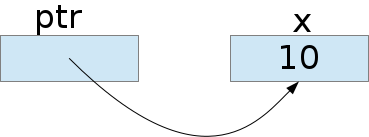
\includegraphics[width=150pt]{imgs/ponteiro.png}
\end{figure}
\item Imprime :
\begin{verbatim}
ptr = 10
Endereco ptr = 0x7ffc2b783634
Endereco x = 0x7ffc2b783634
\end{verbatim}
\end{itemize}
\end{frame}

%%%%%%%%%%%%%%%%%%%%%%%%%%%%%%%%%%%%%%%%%%%%%%%%%%%%%%%%%%%%%%%%%%%%%%%%%%%%%%%%%%%%%%%%%%%%%%%%%%%%%%%%%%%%%%%%%%

\begin{frame}[fragile]
\frametitle{Exemplo}
\begin{lstlisting}
// a, b e c sao variaveis locais, alocadas estaticamente
int a = 10, b = 20, c; 
int *p, *q;  // p e q sao ponteiros que apontam para um inteiro
p = &a;  // o valor de p eh o endereco de a
q = &b;  // q aponta para b
c = *p + *q;  // c recebe o 10 + 20.
\end{lstlisting} 
\end{frame}

%%%%%%%%%%%%%%%%%%%%%%%%%%%%%%%%%%%%%%%%%%%%%%%%%%%%%%%%%%%%%%%%%%%%%%%%%%%%%%%%%%%%%%%%%%%%%%%%%%%%%%%%%%%%%%%%%%

\begin{frame}[fragile]
\frametitle{Exemplo}
\begin{lstlisting}
int a = 10; // a eh alocada estaticamente
int *p; // p eh um ponteiro que aponta para um inteiro
p = &a;  // o valor de p eh o endereco de a
*p = *p + 1; // Incrementa em 1 o valor para o qual p aponta
printf(``a = %d'', a); // Imprime a = 11.
\end{lstlisting} 
\end{frame}

%%%%%%%%%%%%%%%%%%%%%%%%%%%%%%%%%%%%%%%%%%%%%%%%%%%%%%%%%%%%%%%%%%%%%%%%%%%%%%%%%%%%%%%%%%%%%%%%%%%%%%%%%%%%%%%%%%

\begin{frame}
\frametitle{Exercício}
Implemente um função que troque os valores de duas variáveis inteiras. Para isso, a função deve receber o endereço de duas variáveis, a fim de trocar o conteúdo das variáveis originais, e não apenas da cópia local.
\end{frame}

%%%%%%%%%%%%%%%%%%%%%%%%%%%%%%%%%%%%%%%%%%%%%%%%%%%%%%%%%%%%%%%%%%%%%%%%%%%%%%%%%%%%%%%%%%%%%%%%%%%%%%%%%%%%%%%%%%

\begin{frame}[fragile]{Solução}
\begin{lstlisting}
void troca (int *p, int *q)
{
   int temp;
   temp = *p; 
   *p = *q; 
   *q = temp;
}
\end{lstlisting} 
\end{frame}

%%%%%%%%%%%%%%%%%%%%%%%%%%%%%%%%%%%%%%%%%%%%%%%%%%%%%%%%%%%%%%%%%%%%%%%%%%%%%%%%%%%%%%%%%%%%%%%%%%%%%%%%%%%%%%%%%%
\section{Organização da Memória}
%%%%%%%%%%%%%%%%%%%%%%%%%%%%%%%%%%%%%%%%%%%%%%%%%%%%%%%%%%%%%%%%%%%%%%%%%%%%%%%%%%%%%%%%%%%%%%%%%%%%%%%%%%%%%%%%%%

\begin{frame}
\frametitle{Alocação Estática x Alocação Dinâmica}
\begin{itemize}
\item As vezes queremos queremos criar variáveis durante a execução.
\item Mas por quê não declarar variáveis locais?
\begin{itemize}
\item Não sabemos quantas variáveis e quando declará-las.
\item Uma função pode ter que criar uma variável para outras funções usarem.
\item Queremos usar uma organização mais complexa da memória (estrutura de dados).
\end{itemize}
\end{itemize}
\end{frame}

%%%%%%%%%%%%%%%%%%%%%%%%%%%%%%%%%%%%%%%%%%%%%%%%%%%%%%%%%%%%%%%%%%%%%%%%%%%%%%%%%%%%%%%%%%%%%%%%%%%%%%%%%%%%%%%%%%

\begin{frame}[fragile]
\frametitle{Alocação Estática x Alocação Dinâmica}
\begin{itemize}
\item Alocação Estática
\begin{itemize}
\item O espaço para as variáveis é reservado e liberado automaticamente pelo compilador.
\item Exemplo:
\begin{lstlisting}
int a; int b[20];
\end{lstlisting}
\end{itemize}
\item Alocação Dinâmica
\begin{itemize}
\item O espaço para as variáveis é reservado e liberado dinamicamente pelo programador.
\item Para isso, utiliza-se os comandos: malloc(), calloc() e resize().
\item Antes do término do programa, é necessário liberar a memória alocada.
\item Para isso, utiliza-se o comando free().
\end{itemize}
\end{itemize}
\end{frame}

%%%%%%%%%%%%%%%%%%%%%%%%%%%%%%%%%%%%%%%%%%%%%%%%%%%%%%%%%%%%%%%%%%%%%%%%%%%%%%%%%%%%%%%%%%%%%%%%%%%%%%%%%%%%%%%%%%

\begin{frame}[fragile]
\frametitle{Função malloc()}
\begin{itemize}
\item A função  malloc  aloca um bloco de bytes consecutivos na memória RAM e devolve o endereço desse bloco.  
\item No seguinte fragmento de código, aloca-se 1 byte: 
\begin{lstlisting}
char *ptr = malloc( 1 );
\end{lstlisting}
\item Para alocar valores maiores, pode-se recorrer ao operador sizeof, que diz quantos bytes um determinado tipo ocupa. Exemplo:
\begin{lstlisting}
int *ptr = malloc( sizeof( int ) );
\end{lstlisting}
\end{itemize}
\end{frame}

%%%%%%%%%%%%%%%%%%%%%%%%%%%%%%%%%%%%%%%%%%%%%%%%%%%%%%%%%%%%%%%%%%%%%%%%%%%%%%%%%%%%%%%%%%%%%%%%%%%%%%%%%%%%%%%%%%\\

\begin{frame}[fragile]
\frametitle{Função calloc()}
\begin{itemize}
\item A função calloc recebe como parâmetro o número de blocos de memória a serem alocados e o tamanho em bytes de cada bloco. Esse comando aloca a quantidade de memória atribuindo zero a todos os bits.
\item Exemplo: alocar 1 inteiro:
\begin{lstlisting}
int *p;
p = calloc(1, sizeof( int ) );
\end{lstlisting}
\end{itemize}
\end{frame}

%%%%%%%%%%%%%%%%%%%%%%%%%%%%%%%%%%%%%%%%%%%%%%%%%%%%%%%%%%%%%%%%%%%%%%%%%%%%%%%%%%%%%%%%%%%%%%%%%%%%%%%%%%%%%%%%%%

\begin{frame}[fragile]
\frametitle{Função free()}
\begin{itemize}
\item A função free desaloca a porção de memória alocada por malloc() ou calloc(). 
\item A instrução free (ptr) avisa ao sistema que o bloco de bytes apontado por ptr está livre e disponível para reciclagem. Exemplo:
\begin{lstlisting}
int *ptr;
ptr = malloc( sizeof( int ) );
free(ptr);
\end{lstlisting}
\end{itemize}
\end{frame}

%%%%%%%%%%%%%%%%%%%%%%%%%%%%%%%%%%%%%%%%%%%%%%%%%%%%%%%%%%%%%%%%%%%%%%%%%%%%%%%%%%%%%%%%%%%%%%%%%%%%%%%%%%%%%%%%%%

\begin{frame}[fragile]
\frametitle{Memória Disponível}
\begin{itemize}
\item Ao alocar memória, recomenda-se testar se há memória disponível. 
\item Caso não haja a função malloc() e calloc() retornam NULL. Exemplo:
\begin{lstlisting}
int *ptr;
ptr = malloc(sizeof(int));
if (ptr == NULL) {
  printf("Nao ha mais memoria!\n");
  exit(0);
}
*ptr = 13;
printf("Endereco %p com valor %d.\n", ptr, *ptr);
free(ptr);
\end{lstlisting} 
Imprime:\\
Endereco 0x23cd010 com valor 13.
\end{itemize}
\end{frame}

%%%%%%%%%%%%%%%%%%%%%%%%%%%%%%%%%%%%%%%%%%%%%%%%%%%%%%%%%%%%%%%%%%%%%%%%%%%%%%%%%%%%%%%%%%%%%%%%%%%%%%%%%%%%%%%%%%

\begin{frame}
\frametitle{Alocação Dinâmica}
Regras da Alocação Dinâmica
\begin{itemize}
\item Devemos incluir a biblioteca stdlib.h.
\item O tamanho gasto por um tipo pode ser obtido com sizeof().
\item Devemos informar o tamanho a ser reservado para malloc().
\item Devemos verificar se acabou a memória comparando com NULL.
\item Devemos sempre liberar a memória após a utilização com free().
\end{itemize}
\end{frame}

%%%%%%%%%%%%%%%%%%%%%%%%%%%%%%%%%%%%%%%%%%%%%%%%%%%%%%%%%%%%%%%%%%%%%%%%%%%%%%%%%%%%%%%%%%%%%%%%%%%%%%%%%%%%%%%%%%

\begin{frame}
\frametitle{Pilha e Heap}
\begin{itemize}
\item A memória de um programa é dividida em duas partes:
\begin{itemize}
\item Pilha: Onde são armazenadas as variáveis locais, alocadas estaticamente.
\item Heap: Onde são armazenadas as variáveis alocadas dinamicamente, usando malloc(), calloc() ou resize().
\end{itemize}
\end{itemize}
\end{frame}

%%%%%%%%%%%%%%%%%%%%%%%%%%%%%%%%%%%%%%%%%%%%%%%%%%%%%%%%%%%%%%%%%%%%%%%%%%%%%%%%%%%%%%%%%%%%%%%%%%%%%%%%%%%%%%%%%%\\

\begin{frame}
\frametitle{Pilha e Heap}
Pilha
\begin{itemize}
\item Ao declarar uma variável local, o compilador reserva um espaço na pilha.
\item Ao realizar chamadas de funções, os valores são empilhados.
\item O espaço reservado para uma variável local é liberado quando a função termina.
\end{itemize}
\end{frame}

%%%%%%%%%%%%%%%%%%%%%%%%%%%%%%%%%%%%%%%%%%%%%%%%%%%%%%%%%%%%%%%%%%%%%%%%%%%%%%%%%%%%%%%%%%%%%%%%%%%%%%%%%%%%%%%%%%

\begin{frame}
\frametitle{Pilha e Heap}
Heap
\begin{itemize}
\item Ao alocar memória utilizando o comando malloc() ou calloc(), o compilador reserva um espaço no heap, em tempo de execução ({\it runtime}).
\item O espaço reservado usando malloc() deve ser liberado manualmente pelo programador, caso contrário, acontece uma falha de sistema denominada vazamento de memória ({\it memory leak}).
\item O programa valgrind ajuda a detectar vazamentos de memória.
\end{itemize}
\end{frame}

%%%%%%%%%%%%%%%%%%%%%%%%%%%%%%%%%%%%%%%%%%%%%%%%%%%%%%%%%%%%%%%%%%%%%%%%%%%%%%%%%%%%%%%%%%%%%%%%%%%%%%%%%%%%%%%%%%

\begin{frame}
\frametitle{Pilha e Heap}
Representação da Memória
\begin{figure}[!ht]
  \centering
  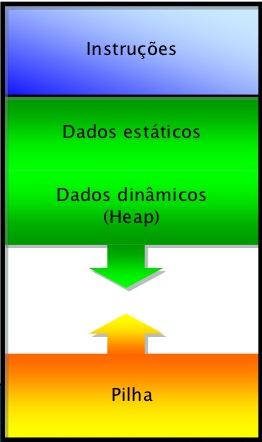
\includegraphics[width=100pt]{imgs/memoria.jpg}
\end{figure}
\end{frame}

%%%%%%%%%%%%%%%%%%%%%%%%%%%%%%%%%%%%%%%%%%%%%%%%%%%%%%%%%%%%%%%%%%%%%%%%%%%%%%%%%%%%%%%%%%%%%%%%%%%%%%%%%%%%%%%%%%
\section{Manipulação da Memória}
%%%%%%%%%%%%%%%%%%%%%%%%%%%%%%%%%%%%%%%%%%%%%%%%%%%%%%%%%%%%%%%%%%%%%%%%%%%%%%%%%%%%%%%%%%%%%%%%%%%%%%%%%%%%%%%%%%

\begin{frame}
\frametitle{Alocação Dinâmica}
\begin{itemize}
\item Também é possível alocar dinamicamente uma quantidade de memória contígua e associá-la com um ponteiro.
\item Desta forma podemos criar programas sem saber a priori o número de dados a ser armazenado.
\item A seguir, um exemplo de alocação dinâmica de um vetor.
\end{itemize}
\end{frame}

%%%%%%%%%%%%%%%%%%%%%%%%%%%%%%%%%%%%%%%%%%%%%%%%%%%%%%%%%%%%%%%%%%%%%%%%%%%%%%%%%%%%%%%%%%%%%%%%%%%%%%%%%%%%%%%%%%

\begin{frame}[fragile]
\frametitle{Exemplo: alocação de vetor}
\begin{lstlisting}
int *vetor, i, n;
scanf("%d", &n);
vetor = malloc(n * sizeof( int ) );
for (i = 0; i < n; i++)
  scanf("%d", &vetor[i] );
free(vetor);
\end{lstlisting} 
\end{frame}

%%%%%%%%%%%%%%%%%%%%%%%%%%%%%%%%%%%%%%%%%%%%%%%%%%%%%%%%%%%%%%%%%%%%%%%%%%%%%%%%%%%%%%%%%%%%%%%%%%%%%%%%%%%%%%%%%%

\begin{frame}[fragile]
\frametitle{Aritmética de ponteiros}
\begin{itemize}
\item Podemos realizar operações aritméticas em ponteiros: soma, subtração, incremento e decremento.
\item No entanto, ao realizar essas operações, estaremos realizando deslocamentos no endereço. Exemplo:
\end{itemize}
\begin{lstlisting}
  int vetor[] = {1, 2, 3, 4, 5}, *ptr;
  ptr = vetor + 2;
  printf("ptr: %d\n", *ptr);
  ptr++;
  printf("ptr: %d\n", *ptr);
\end{lstlisting} 
\begin{figure}[!ht]
  \centering
  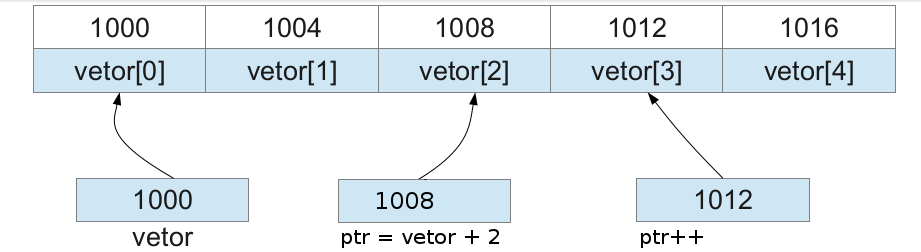
\includegraphics[width=300pt]{imgs/aritmetica_ponteiro.png}
\end{figure}
\end{frame}

%%%%%%%%%%%%%%%%%%%%%%%%%%%%%%%%%%%%%%%%%%%%%%%%%%%%%%%%%%%%%%%%%%%%%%%%%%%%%%%%%%%%%%%%%%%%%%%%%%%%%%%%%%%%%%%%%%

\begin{frame}
  \frametitle{Exercícios}
\begin{itemize}
\item Escreva uma função que compara duas strings e retorna 1 se a primeira string vier antes da segunda na ordem alfabética.
\end{itemize}
\end{frame}

%%%%%%%%%%%%%%%%%%%%%%%%%%%%%%%%%%%%%%%%%%%%%%%%%%%%%%%%%%%%%%%%%%%%%%%%%%%%%%%%%%%%%%%%%%%%%%%%%%%%%%%%%%%%%%%%%%
\section{Ponteiros Duplos}
%%%%%%%%%%%%%%%%%%%%%%%%%%%%%%%%%%%%%%%%%%%%%%%%%%%%%%%%%%%%%%%%%%%%%%%%%%%%%%%%%%%%%%%%%%%%%%%%%%%%%%%%%%%%%%%%%%

\begin{frame}[fragile]
\frametitle{Ponteiros para ponteiros}
\begin{itemize}
\item  Uma variável ponteiro está alocada na memória do computador como qualquer outra variável.
\item Portanto podemos criar um ponteiro que contém o endereço de memória de um outro ponteiro.
\item Para criar um ponteiro duplo, ou seja, um ponteiro para outro ponteiro: tipo \verb|**nomePonteiro|.
\end{itemize}
\begin{lstlisting}
int a=5, *b, **c;
b = &a;
c = &b;
printf("%d\n", a);
printf("%d\n", *b);
printf("%d\n", *(*c));
\end{lstlisting}
\end{frame}

%%%%%%%%%%%%%%%%%%%%%%%%%%%%%%%%%%%%%%%%%%%%%%%%%%%%%%%%%%%%%%%%%%%%%%%%%%%%%%%%%%%%%%%%%%%%%%%%%%%%%%%%%%%%%%%%%%

\begin{frame}
\frametitle{Ponteiros para Ponteiros}
\begin{itemize}
\item O programa imprime 5 três vezes, monstrando as três formas de acesso à variável a: a, *b, **c.
\end{itemize}
\begin{figure}[!ht]
  \centering
  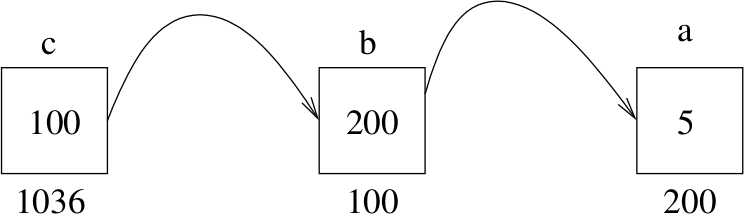
\includegraphics[width=200pt]{imgs/ponteiro_duplo.png}
\end{figure}
\end{frame}

%%%%%%%%%%%%%%%%%%%%%%%%%%%%%%%%%%%%%%%%%%%%%%%%%%%%%%%%%%%%%%%%%%%%%%%%%%%%%%%%%%%%%%%%%%%%%%%%%%%%%%%%%%%%%%%%%%

\begin{frame}[fragile]
\frametitle{Ponteiros para Ponteiros}
\begin{itemize}
\item A mesma coisa acontece se declararmos um vetor de ponteiros duplos.
\begin{lstlisting}
int **p;
p = calloc(5,  sizeof( int *) );
\end{lstlisting}
\item Teremos um vetor, onde cada posição do vetor é do tipo int *, ou seja, é um ponteiro para um inteiro.
\begin{figure}[!ht]
  \centering
  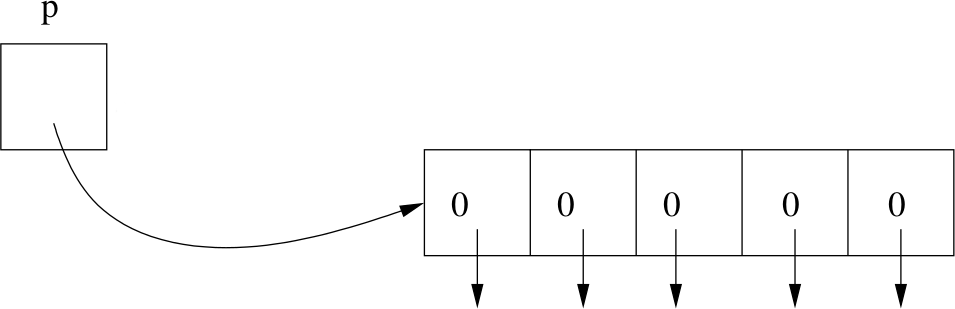
\includegraphics[width=200pt]{imgs/vetor_de_ponteiros.png}
\end{figure}
\end{itemize}
\end{frame}

%%%%%%%%%%%%%%%%%%%%%%%%%%%%%%%%%%%%%%%%%%%%%%%%%%%%%%%%%%%%%%%%%%%%%%%%%%%%%%%%%%%%%%%%%%%%%%%%%%%%%%%%%%%%%%%%%%

\begin{frame}[fragile]
\frametitle{Ponteiros para Ponteiros}
\begin{itemize}
\item Como cada posição do vetor é um ponteiro para inteiro, podemos
associar cada posição dinamicamente com um vetor de inteiros!
\begin{lstlisting}
int **p;
int i;
p = calloc(5, sizeof(int *) );
for(i=0; i<5; i++)
  p[i] = calloc(3, sizeof( int ) );
\end{lstlisting}
\item Dessa forma, teremos uma matriz alocada dinamicamente.
\begin{figure}[!ht]
  \centering
  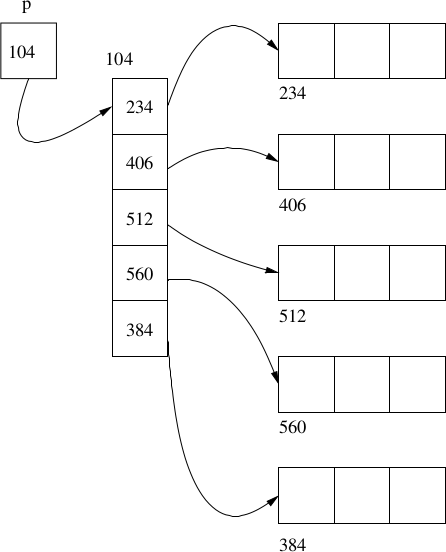
\includegraphics[width=75pt]{imgs/matriz_dinamica.png}
\end{figure}
\end{itemize}
\end{frame}

%%%%%%%%%%%%%%%%%%%%%%%%%%%%%%%%%%%%%%%%%%%%%%%%%%%%%%%%%%%%%%%%%%%%%%%%%%%%%%%%%%%%%%%%%%%%%%%%%%%%%%%%%%%%%%%%%%

\begin{frame}
  \frametitle{Matriz Dinâmica}
Esta é a forma de se criar matrizes dinamicamente:
\begin{itemize}
\item Crie um ponteiro para ponteiro. 
\item Associe um vetor de ponteiros dinamicamente com este ponteiro de
ponteiro. O tamanho deste vetor é o número de linhas da matriz.
\item Cada posição do vetor será associado com um outro vetor do tipo a
ser armazenado. Cada um destes vetores é uma linha da matriz (portanto possui tamanho igual ao número de colunas).
\end{itemize}
\begin{figure}[!ht]
  \centering
  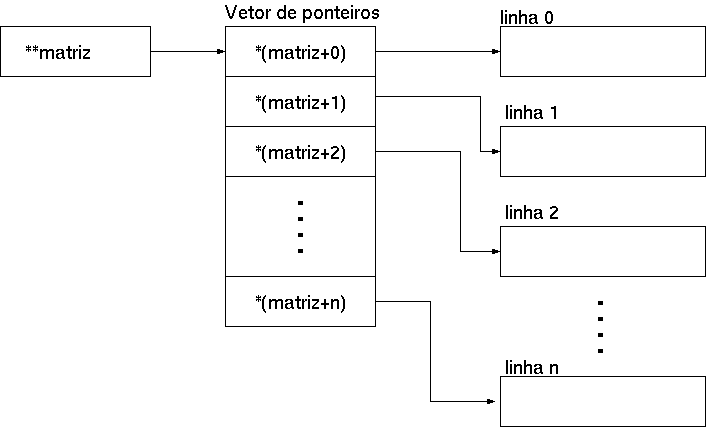
\includegraphics[width=180pt]{imgs/matriz_dinamica2.png}
\end{figure}
\end{frame}

%%%%%%%%%%%%%%%%%%%%%%%%%%%%%%%%%%%%%%%%%%%%%%%%%%%%%%%%%%%%%%%%%%%%%%%%%%%%%%%%%%%%%%%%%%%%%%%%%%%%%%%%%%%%%%%%%%

\begin{frame}[fragile]
\frametitle{Matriz Dinâmica}
\begin{itemize}
\item No final você deve desalocar toda a memória alocada.
\item Para desalocar toda a memória alocada, percorre-se cada linha da matriz liberando a memória.
\begin{lstlisting}
  int **m = calloc(5, sizeof(int *));
  for (int i = 0; i < 5; i++)
    m[i] = calloc(5, sizeof(int));
  ...
  for (int i = 0; i < 5; i++)
    free(m[i]);
  free(m);
\end{lstlisting}
\end{itemize}
\end{frame}

%%%%%%%%%%%%%%%%%%%%%%%%%%%%%%%%%%%%%%%%%%%%%%%%%%%%%%%%%%%%%%%%%%%%%%%%%%%%%%%%%%%%%%%%%%%%%%%%%%%%%%%%%%%%%%%%%%

\begin{frame}
  \frametitle{Exercícios}
\begin{itemize}
\item Escreva um programa que leia uma quantidade arbitrária de nomes e imprima esses nomes em ordem alfabética
\end{itemize}
\end{frame}

%%%%%%%%%%%%%%%%%%%%%%%%%%%%%%%%%%%%%%%%%%%%%%%%%%%%%%%%%%%%%%%%%%%%%%%%%%%%%%%%%%%%%%%%%%%%%%%%%%%%%%%%%%%%%%%%%%

\begin{frame}
\frametitle{Exercício}
Crie um programa que multiplica duas matrizes quadradas do tipo double lidas do teclado. Seu programa de ler a dimensão n da matriz, em seguida alocar dinamicamente duas matrizes $n \times n$. Depois ler os dados das duas matrizes e imprimir a matriz resultante da multiplicação destas.
\end{frame}

%%%%%%%%%%%%%%%%%%%%%%%%%%%%%%%%%%%%%%%%%%%%%%%%%%%%%%%%%%%%%%%%%%%%%%%%%%%%%%%%%%%%%%%%%%%%%%%%%%%%%%%%%%%%%%%%%%

\begin{frame}
\frametitle{Conclusão}
\begin{itemize}
\item Nesta aula foram apresentados conceitos e exemplos de alocação dinâmica de mémoria.
\item Pontos de maior atenção para alocação e liberação de memória e passagem de parâmetros por valor e referência.
\item Em seus programas você deverá estar atento ao momento
exato de liberação da memória.
\item Tipos Abstratos de Dados (TADs).
\end{itemize}
\end{frame}

%%%%%%%%%%%%%%%%%%%%%%%%%%%%%%%%%%%%%%%%%%%%%%%%%%%%%%%%%%%%%%%%%%%%%%%%%%%%%%%%%%%%%%%%%%%%%%%%%%%%%%%%%%%%%%%%%%

\begin{frame}{Material Recomendado}
\begin{itemize}
\item DEITEL, Paul; DEITEL, Harvey. C: Como Programar. Capítulo 7. Pearson, 6ª ed. 2011. \textcolor{blue}{ \href{http://www.inf.ufsc.br/~bosco.sobral/ensino/ine5201-02202A/Deitel_-_C_Como_programar_-_6a_edicao.pdf}{Disponível aqui}. } 
\item Tutorial de uso do software Valgrind. \textcolor{blue}{ \href{https://www.ic.unicamp.br/~rafael/materiais/valgrind.html}{Disponível aqui}. } 
\end{itemize}
\end{frame}

%%%%%%%%%%%%%%%%%%%%%%%%%%%%%%%%%%%%%%%%%%%%%%%%%%%%%%%%%%%%%%%%%%%%%%%%%%%%%%%%%%%%%%%%%%%%%%%%%%%%%%%%%%%%%%%%%%

\end{document}
